% AI-Based Time Series Weather Data Validation Platform
% IEEE two-column conference format (IEEEtran). Build: pdflatex paper.tex (twice).
% All fault results are on SYNTHETIC faults, held-out validation years 2013--2017, seed 42.
\documentclass[conference,a4paper]{IEEEtran}

\usepackage[T1]{fontenc}
\usepackage{times}
\usepackage{amsmath,amssymb}
\usepackage{graphicx}
\usepackage{booktabs}
\usepackage{cite}
\usepackage{url}
\usepackage{microtype}
\graphicspath{{figures/}}

\hyphenation{Data-Mend Weather ConvGRU}

\begin{document}

\title{AI-Based Time Series Weather Data\\Validation Platform}

\author{%
\IEEEauthorblockN{Nathasha Lewis}
\IEEEauthorblockA{Dept.\ of Computer Engineering\\
Fr.\ Conceicao Rodrigues College of Engineering\\
Mumbai, India}
\and
\IEEEauthorblockN{Anshu Jadhav}
\IEEEauthorblockA{Dept.\ of Computer Engineering\\
Fr.\ Conceicao Rodrigues College of Engineering\\
Mumbai, India}
\and
\IEEEauthorblockN{Rochelle Fernandes}
\IEEEauthorblockA{Dept.\ of Computer Engineering\\
Fr.\ Conceicao Rodrigues College of Engineering\\
Mumbai, India}
\and
\IEEEauthorblockN{Guide: Prof.\ Jagruti Nagaonkar}
\IEEEauthorblockA{Dept.\ of Computer Engineering\\
Fr.\ Conceicao Rodrigues College of Engineering\\
University of Mumbai, India}}

\maketitle

\begin{abstract}
Rainfall records underpin flood warning, agriculture and climate research, yet every record contains faulty values such as stuck gauges, spikes, scaling errors and phantom rain. This paper presents DataMend, an AI-based validation platform that accepts a rainfall time series from a file, a live gauge feed or a gridded product and returns a verdict for every value together with the evidence behind it. The platform combines a transparent catalogue of eight reading checks and four daily checks, each declaring its inputs and reporting explicitly when it cannot run, with STNet, a compact spatio-temporal network (1.76 million parameters) trained on the 0.25-degree IMD RF25 grid. STNet couples a convolutional spatial encoder with a ConvGRU memory and three output heads, and its scores are fused with the rules at a fixed budget of one false alarm per 1,000 clean cell-days. On a frozen benchmark of six synthetic fault families in held-out validation years, a linear probe on STNet features separates every family with an AUC between 0.888 and 0.999, and the fused detector reaches a PR-AUC of 0.691 and a recall of 0.635 while flagging only 0.6\% of protected heavy-rain cell-days. The system is delivered as a FastAPI backend and a React dashboard, is verified by 569 automated tests and follows an evaluation protocol that fixes budgets on validation data before any test year is scored.
\end{abstract}

\begin{IEEEkeywords}
rainfall quality control, time-series validation, spatio-temporal neural networks, anomaly detection, explainable flags, IMD RF25
\end{IEEEkeywords}

%% ------------------------------------------------------------------------------------------------
\section{Introduction}
Rainfall is the most consequential and the most irregular of the weather variables. It is zero on most days and strongly skewed on the rest, so a single erroneous value can change a flood model, an agricultural advisory or a climate trend. Gauges jam and repeat one reading for weeks, loggers write zeros during faults, transmission errors scale values by an order of magnitude, and interpolation spreads one bad gauge across its neighbours. Detecting such errors before the data are used is the task of quality control (QC) \cite{durre2010,chandola2009}.

Operational QC rests on long lists of fixed tests and manual review \cite{durre2010}, while learned detectors that exploit spatial context have recently been shown to improve precipitation QC \cite{sha2021}. A practical gap remains: a single, reproducible system that takes a rainfall series from any source, applies both rule-based and learned evidence, explains every flag and records exactly what was done. Two requirements make the problem distinctive. First, an unusual value is not necessarily a wrong value, because the heaviest rainfall is also the most valuable, so extremes must be separated from faults. Second, every flag has an operational cost, so performance must be stated at an explicit false-alarm budget rather than as accuracy.

This paper presents DataMend, a rainfall validation platform with two parts: a validation platform (Part~A) and a trained model system, STNet (Part~B), operating on the 0.25-degree IMD RF25 daily grid \cite{pai2014}. The contributions are:
\begin{itemize}
\item A layered validation platform with a strict input contract, a catalogue of eight reading and four daily checks that declare their needs and report ``not run'' explicitly, stored runs, JSON and CSV reports, an explainer interface and a reviewer loop.
\item STNet, a compact spatio-temporal fault detector (1.76 million parameters, 6.8~MB) with fault, clean and discrimination heads that separates genuine extremes from faults.
\item A fusion and calibration scheme that fixes the flag threshold from validation curves at a stated false-alarm budget and reports the rate at which protected extremes are flagged.
\item A frozen, reproducible evaluation protocol on six synthetic fault families, with 569 automated tests supporting the implementation.
\end{itemize}
The remainder of the paper is organised as follows. Section~\ref{sec:related} reviews related work, Section~\ref{sec:design} describes the system design, Section~\ref{sec:impl} the implementation, Section~\ref{sec:eval} the evaluation, Section~\ref{sec:disc} discusses the results and Section~\ref{sec:concl} concludes.

%% ------------------------------------------------------------------------------------------------
\section{Related Work}\label{sec:related}
\subsection{Rule-Based Quality Control}
Durre et al.\ describe the automated quality assurance of the Global Historical Climatology Network-Daily data set: duplicate and impossible values, outliers against station climatology, temporal persistence, internal consistency and spatial comparison, validated manually and flagging 0.24\% of more than 1.5 billion values \cite{durre2010}. Such systems are transparent and inexpensive, and they define the vocabulary of checks that the DataMend catalogue adopts. Their thresholds are set by hand, which motivates adding a calibrated, budgeted learned layer.

\subsection{Learned Detectors}
Chandola et al.\ organise anomaly detection by data type and learning setting \cite{chandola2009}. Recurrent models such as LSTM \cite{hochreiter1997} and GRU \cite{cho2014} predict or reconstruct series, and convolutional recurrent networks carry the idea to gridded fields by replacing matrix products with convolutions \cite{shi2015}. Sha et al.\ applied convolutional networks to gridded precipitation and elevation fields to quality-control gauge observations and reported an AUC of 0.927 \cite{sha2021}, demonstrating the value of spatial context. STNet follows this direction with a convolutional encoder for the spatial neighbourhood and a ConvGRU for temporal memory.

\subsection{Federated and Distributed Learning}
Federated learning trains a model across data holders by exchanging parameters rather than data \cite{mcmahan2017,kairouz2021}. FedProx \cite{li2020prox} and FedPer \cite{arivazhagan2019} address non-identical clients and Li et al.\ survey the open problems \cite{li2020sp}. Federated fault detection has been demonstrated for sensor networks \cite{khan2024}, weather forecasting \cite{chen2023} and as a time-series benchmark \cite{liu2022}. The DataMend model system defines eight regional clients composed of whole IMD sub-divisions, which keeps the design ready for settings in which regional data cannot be pooled.

\subsection{Positioning}
DataMend builds on these strands through their integration: layered validation with explicit not-run reporting, discrimination of genuine extremes from faults, evidence behind every flag, an explanation seam and an evaluation anchored to a fixed false-alarm budget. The data sources are the IMD RF25 grid \cite{pai2014}, the Weather Union gauge network \cite{weatherunion} and station metadata derived from NOAA's Integrated Surface Database history file \cite{noaaisd}.

%% ------------------------------------------------------------------------------------------------
\section{System Design}\label{sec:design}
\subsection{Architecture}
Fig.~\ref{fig:arch} shows the system. A series enters through the input contract, passes the check catalogue and leaves as per-row verdicts, scores and evidence collected in a stored run report. A score-provider seam accepts a calibrated trained score from Part~B, and an explainer interface serves a rule-based baseline and an external AI narrator. Two invariants hold throughout: the original data are never overwritten, and the narrator never changes a verdict, score or evidence.

\begin{figure*}[!t]
\centering
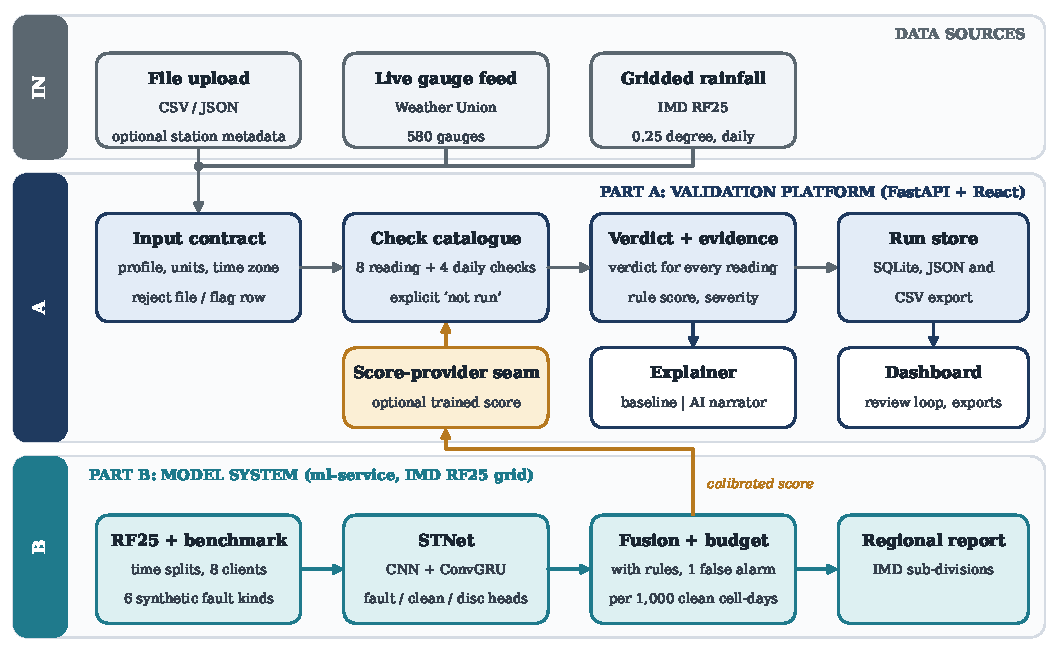
\includegraphics[width=0.86\textwidth]{fig_architecture.pdf}
\caption{Architecture of DataMend: data sources, validation platform (Part~A) and model system (Part~B).}
\label{fig:arch}
\end{figure*}

\subsection{Input Contract and Check Catalogue}
The input contract accepts CSV and JSON in a reading profile or a daily profile. A file-level problem rejects the file, whereas a row-level problem (missing, negative, non-numeric, duplicated or out-of-order values) keeps the row with a flag and a reason. The catalogue contains eight reading checks, four daily checks and duplicate-row detection. Each check declares the inputs it needs, so a check that cannot run, for example a neighbour check without neighbours, is listed as not run instead of silently passing. Each row receives a verdict (OK, SUSPECT, UNCERTAIN or NO\_DATA), an uncalibrated rule score with a severity band and evidence tagged as measured, assumed or derived.

\subsection{Evidence, Explanation and Review}
Evidence follows a versioned JSON contract (evidence-v1) with a window cap of 24 readings or 14 days and a 64~KB size cap. An explainer interface produces explanations from the stored evidence; a rule-based baseline is always available, and an external AI narrator can be attached behind the same interface. Explanations are stored separately and always marked as generated. Reviewers record decisions (confirmed fault, false alarm, genuine extreme or needs follow-up) that are stored apart from the evidence and never alter a verdict.

\subsection{STNet}
STNet reads a window of consecutive daily rainfall fields. A convolutional encoder (width 32, 16 features) summarises each cell's spatial neighbourhood, a ConvGRU carries temporal memory and an optional long-range LSTM branch provides seasonal memory. Three heads share the representation: a fault head scores each cell-day for faults, a clean head scores plausibility and a discrimination head separates genuine extremes from faults. A robust input transform handles the heavy tail of rainfall. Training weights fault cell-days with 10, protected extremes with 3 and ambiguous extremes with 2. The network has 1,761,769 parameters (6.8~MB) and requires 8.2~GFLOPs per day over the full grid.

\subsection{Fusion and False-Alarm Budget}
For a cell-day $i$, the rule score $r_i$ and the STNet fault score $s_i$ are fused by a logistic layer,
\begin{equation}
p_i = \sigma\!\left(\beta_0 + \beta_r\, r_i + \beta_s\, s_i\right),
\label{eq:fusion}
\end{equation}
where $\beta$ are learned weights; a boosted variant is evaluated in parallel. For a budget $b$, the threshold $\tau$ is the smallest value for which the false-alarm rate on the clean set $C$ does not exceed $b$,
\begin{equation}
\mathrm{FA}(\tau) = 1000\cdot\frac{\left|\{\,i\in C : p_i > \tau\,\}\right|}{|C|} \le b,
\label{eq:budget}
\end{equation}
with $b=1$ in this work. Recall is then the share of the fault set $F$ whose fused probability exceeds $\tau$. The rule score and the calibrated flag are never mixed in one number.

%% ------------------------------------------------------------------------------------------------
\section{Implementation}\label{sec:impl}
The backend is written in Python with FastAPI, with business logic in services rather than in routes; storage is SQLite with portable JSON columns so that it can move to PostgreSQL. The dashboard is a React and TypeScript application with views for overview, runs, data explorer, review queue, anomaly lab, locations, live gauge feed, station network and settings. The station network view maps 580 Weather Union gauges and 541 Indian synoptic stations, coloured by check, flag and audit state. A live Weather Union feed is scored by the same catalogue as one open run per rain day. Settings editable from the dashboard are protected by an admin token with constant-time comparison and rate limiting, and secrets are write-only. The system is containerised with Docker. The model system is implemented in PyTorch with YAML configurations that fix splits, seeds and the benchmark, and every run records wall time, memory, GPU use and energy.

%% ------------------------------------------------------------------------------------------------
\section{Evaluation}\label{sec:eval}
\subsection{Data, Benchmark and Protocol}
The IMD RF25 daily grid \cite{pai2014} is split by time: earlier years train, validation years 2013--2017 are used for selection and the final years are test years scored once. Eight regional clients are formed from whole IMD sub-divisions so that no sub-division mixes trained and unseen cells, and two clients (3 and 6) are held out. Because expert error labels are not available for the grid, a frozen, hash-checked benchmark corrupts clean data with six fault families (spike, stuck, scale, phantom rain, zeroed and drift), together with protected extremes that are never corrupted and ambiguous single-cell extremes that are tracked separately. Fault results are therefore reported on synthetic faults. Budgets are fixed on validation data only, and each design decision is accepted or declined by a rule written before the run. Metrics are PR-AUC, recall, event recall, false alarms per 1,000 clean cell-days and the share of protected extremes flagged.

\subsection{Separability of Fault Families}
A linear probe fitted on 2013 and tested on 2014 shows that STNet's features separate every fault family from clean data (Fig.~\ref{fig:probe}): AUC is 0.999 for spikes, 0.987 for phantom rain, 0.975 for stuck gauges, 0.938 for scale errors, 0.895 for drift and 0.888 for zeroed values.

\begin{figure}[!t]
\centering
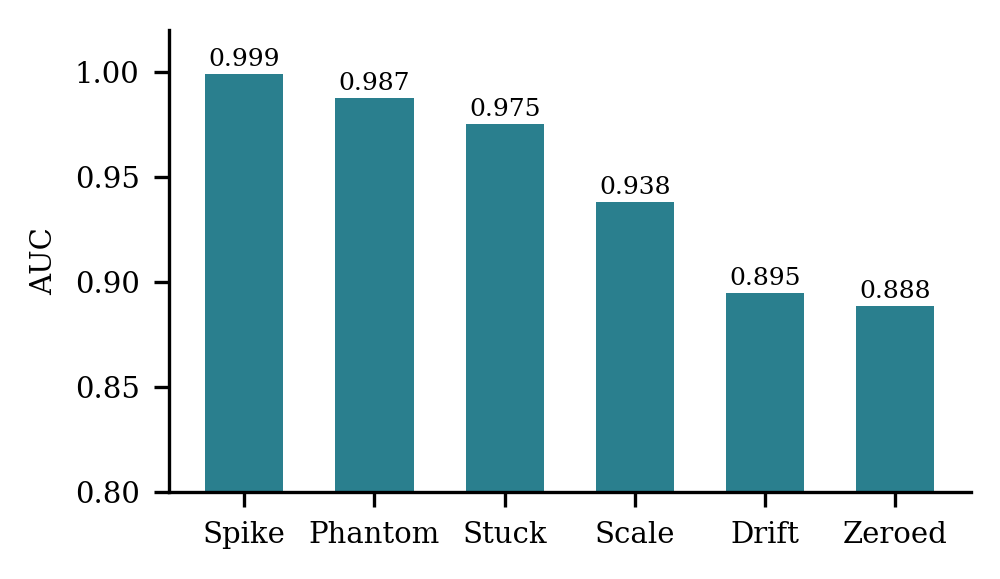
\includegraphics[width=\columnwidth]{pp_probe_auc.png}
\caption{Linear-probe AUC of STNet features by fault family (synthetic faults; fit 2013, test 2014).}
\label{fig:probe}
\end{figure}

\subsection{Operating Point}
Table~\ref{tab:op} gives the results at one false alarm per 1,000 clean cell-days. With the rules and the fault head fused by the logistic layer, the detector reaches a PR-AUC of 0.691, a recall of 0.635, an event recall of 0.619 and an IoU of 0.755, while flagging 0.6\% of protected extremes. Event recall is highest for spikes (0.993), stuck gauges (0.991) and phantom rain (0.957), and the overall event recall of the fault head is 0.659.

\begin{table}[!t]
\caption{Fused rules + STNet at one false alarm per 1,000 clean cell-days (synthetic faults)}
\label{tab:op}
\centering
\footnotesize
\begin{tabular}{@{}lccccc@{}}
\toprule
Variant & PR-AUC & Recall & Event rec. & FA/1,000 & Prot. \\
\midrule
Rules + fault head (logistic) & 0.691 & 0.635 & 0.619 & 1.27 & 0.6\% \\
Rules + fault head (boosted)  & 0.682 & 0.629 & 0.573 & 0.73 & 2.7\% \\
Rules + fault + clean heads   & 0.693 & 0.636 & 0.608 & 1.24 & 1.9\% \\
Rules + four STNet heads      & 0.707 & 0.644 & 0.637 & 1.38 & 2.3\% \\
\bottomrule
\end{tabular}
\end{table}

\subsection{Detection Against Fault Size}
Recall grows monotonically with the size of the fault (Fig.~\ref{fig:recall}), from 0.427 for changes below 0.1~mm to 0.885 for changes of 20--100~mm and 0.896 above 100~mm. For strong faults, defined as a change of at least 5~mm with a footprint weight of at least 0.5, the recall is 0.778. These are the faults with the largest operational consequence.

\begin{figure}[!t]
\centering
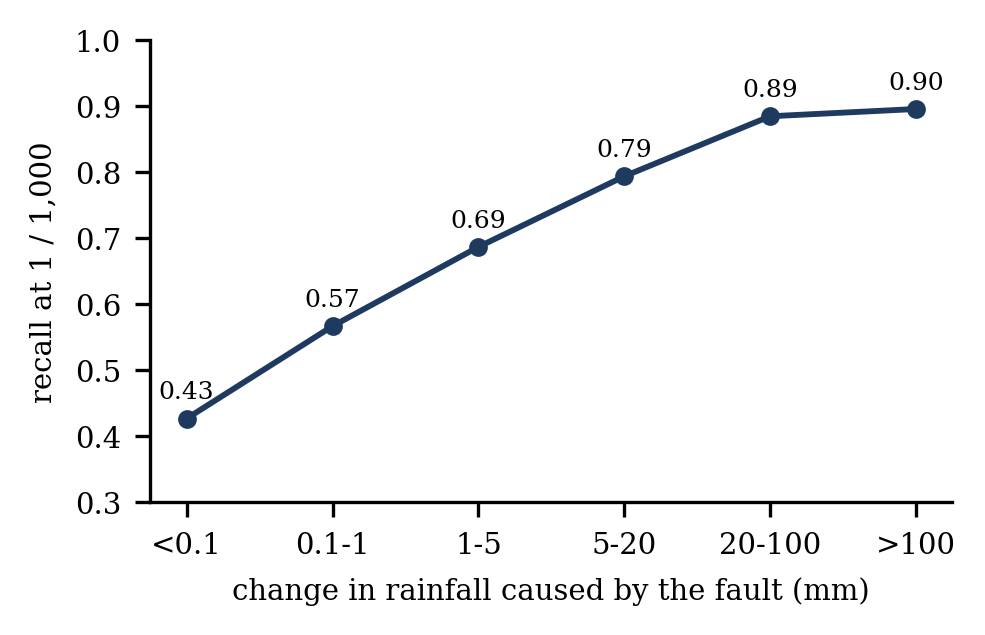
\includegraphics[width=\columnwidth]{pp_recall_vs_size.png}
\caption{Recall of the STNet fault head at one false alarm per 1,000 against the size of the fault.}
\label{fig:recall}
\end{figure}

\subsection{Regional Calibration}
Across the eight regional clients, the calibrated false-alarm rate under the global threshold lies between 0.56 and 1.80 per 1,000 clean cell-days (mean 1.12, derived), with 95\% intervals computed from 358,125 to 484,827 clean cell-days per client; the two held-out regions score 1.80 and 1.15.

\subsection{Design Decisions Under the Protocol}
A paired comparison with a longer-memory encoder, resampled over whole validation years, improved recall by 3.4 points and PR-AUC by 2.1 points, better in all five years, with the largest gains for stuck-gauge faults (recall 0.770 to 0.860) and zeroed faults (event recall 0.282 to 0.366). A candidate cumulative-sum drift stage was evaluated against the fault head under an acceptance rule fixed before the run; it did not meet the rule and was not added, which keeps the delivered pipeline compact.

\subsection{Cost and Verification}
Training STNet took 9,172~s on a single Tesla T4 GPU (165.7~Wh of GPU energy, 5.3~GB peak GPU memory). Network inference runs at about 50 days of the full grid per second. The platform and model system are covered by 239 and 330 automated tests respectively, using generated data and mocked transports, and a seeded anomaly lab injected faults through the real pipeline, with every injected fault flagged across three seeds and both profiles.

%% ------------------------------------------------------------------------------------------------
\section{Discussion}\label{sec:disc}
The results show that a compact network trained on a national grid yields features that separate all six synthetic fault families, and that fusing its score with transparent rules gives a detector that operates at a stated false-alarm budget while rarely flagging protected heavy-rain events. Recall rises with fault magnitude, which matches operational need: the faults that matter most for flood and water-resource decisions are the ones detected most reliably. The layered design also keeps every flag explainable, since the rule evidence is stored with each verdict and the trained score enters only through a defined seam.

The benchmark uses synthetic faults, which provide exact ground truth and controlled stress tests across fault types and magnitudes; the corresponding result on expert-reviewed labels is the natural next step as such labels become available for Indian stations. The frozen protocol, in which budgets are fixed on validation data and test years are scored once, makes every figure reproducible and prevents tuning against the test period.

%% ------------------------------------------------------------------------------------------------
\section{Conclusion and Future Work}\label{sec:concl}
This paper presented DataMend, an AI-based rainfall time-series validation platform that combines an explainable catalogue of checks, a compact spatio-temporal detector and a budgeted fusion scheme. STNet, with 1.76 million parameters, trains in 2.5 hours on one GPU and separates six fault families with an AUC between 0.888 and 0.999; fused with the rules at one false alarm per 1,000 clean cell-days it reaches a PR-AUC of 0.691 and recall of 0.635 while flagging 0.6\% of protected extremes. The platform, with its input contract, runs, explainer seam, live feed, station-network view and reviewer loop, is verified by 569 automated tests.

Future work comprises connecting the trained score to live gauges through the score-provider seam, evaluating on expert-reviewed labels and with multiple seeds, attaching the AI narrator through the documented contract, replaying NOAA ISD history for India, and extending the federated variants to real regional clients. Reliable rainfall records support flood preparedness, food security and climate action, in line with the Sustainable Development Goals \cite{un2015}.

%% ------------------------------------------------------------------------------------------------
\begin{thebibliography}{18}
\bibitem{durre2010} I.~Durre, M.~J. Menne, B.~E. Gleason, T.~G. Houston and R.~S. Vose, ``Comprehensive automated quality assurance of daily surface observations,'' \emph{J. Appl. Meteorol. Climatol.}, vol.~49, no.~8, pp.~1615--1633, 2010.
\bibitem{chandola2009} V.~Chandola, A.~Banerjee and V.~Kumar, ``Anomaly detection: A survey,'' \emph{ACM Comput. Surv.}, vol.~41, no.~3, art.~15, 2009.
\bibitem{sha2021} Y.~Sha, D.~J. Gagne, G.~West and R.~Stull, ``Deep-learning-based precipitation observation quality control,'' \emph{J. Atmos. Ocean. Technol.}, vol.~38, no.~5, pp.~1075--1091, 2021.
\bibitem{pai2014} D.~S. Pai \emph{et al.}, ``Development of a new high spatial resolution ($0.25\times0.25$ degree) long period (1901--2010) daily gridded rainfall data set over India,'' \emph{MAUSAM}, vol.~65, no.~1, pp.~1--18, 2014.
\bibitem{hochreiter1997} S.~Hochreiter and J.~Schmidhuber, ``Long short-term memory,'' \emph{Neural Comput.}, vol.~9, no.~8, pp.~1735--1780, 1997.
\bibitem{cho2014} K.~Cho \emph{et al.}, ``Learning phrase representations using RNN encoder-decoder for statistical machine translation,'' in \emph{Proc. EMNLP}, 2014, pp.~1724--1734.
\bibitem{shi2015} X.~Shi, Z.~Chen, H.~Wang, D.-Y. Yeung, W.-K. Wong and W.-C. Woo, ``Convolutional LSTM network: A machine learning approach for precipitation nowcasting,'' in \emph{Proc. NeurIPS}, 2015, pp.~802--810.
\bibitem{mcmahan2017} B.~McMahan, E.~Moore, D.~Ramage, S.~Hampson and B.~Aguera y Arcas, ``Communication-efficient learning of deep networks from decentralized data,'' in \emph{Proc. AISTATS}, PMLR vol.~54, 2017, pp.~1273--1282.
\bibitem{kairouz2021} P.~Kairouz \emph{et al.}, ``Advances and open problems in federated learning,'' \emph{Found. Trends Mach. Learn.}, vol.~14, no.~1--2, pp.~1--210, 2021.
\bibitem{li2020prox} T.~Li, A.~K. Sahu, M.~Zaheer, M.~Sanjabi, A.~Talwalkar and V.~Smith, ``Federated optimization in heterogeneous networks,'' in \emph{Proc. MLSys}, 2020, arXiv:1812.06127.
\bibitem{arivazhagan2019} M.~G. Arivazhagan, V.~Aggarwal, A.~K. Singh and S.~Choudhary, ``Federated learning with personalization layers,'' arXiv:1912.00818, 2019.
\bibitem{li2020sp} T.~Li, A.~K. Sahu, A.~Talwalkar and V.~Smith, ``Federated learning: Challenges, methods, and future directions,'' \emph{IEEE Signal Process. Mag.}, vol.~37, no.~3, pp.~50--60, 2020.
\bibitem{khan2024} R.~Khan, U.~Saeed and I.~Koo, ``FedLSTM: A federated learning framework for sensor fault detection in wireless sensor networks,'' \emph{Electronics}, vol.~13, no.~24, art.~4907, 2024.
\bibitem{chen2023} S.~Chen, G.~Long, T.~Shen and J.~Jiang, ``Prompt federated learning for weather forecasting: Toward foundation models on meteorological data,'' in \emph{Proc. IJCAI}, 2023, pp.~3532--3540.
\bibitem{liu2022} F.~Liu \emph{et al.}, ``FedTADBench: Federated time-series anomaly detection benchmark,'' arXiv:2212.09518, 2022.
\bibitem{weatherunion} Weather Union, ``Weather Union API documentation,'' \url{https://www.weatherunion.com/dashboard/}, accessed Nov.~19, 2026.
\bibitem{noaaisd} NOAA National Centers for Environmental Information, ``Integrated Surface Database (ISD) readme,'' \url{https://www.ncei.noaa.gov/pub/data/noaa/readme.txt}.
\bibitem{un2015} United Nations General Assembly, ``Transforming our world: the 2030 Agenda for Sustainable Development,'' A/RES/70/1, 2015.
\end{thebibliography}

\end{document}
